\documentclass[13pt]{article}
\usepackage{graphicx}
\usepackage{times}
\usepackage[usenames, dvipsnames]{color}
\usepackage{type1cm}
\usepackage{eso-pic}
\usepackage{color}
\usepackage{ulem}
\usepackage{everypage}
\usepackage{amssymb}
\usepackage[margin=3 cm]{geometry}
%\usepackage[usenames,dvipsnames]{color}
\usepackage{amsmath}




\begin{document}

% Article top matter
\title{\textcolor{BurntOrange}{ Euclid Algorithm }}

\begin{center}
\huge
{\bf \textcolor{ForestGreen}{
{  Hyperdex: a distributed searchable key value store }       \\
}
}
\vspace{2 cm}
\huge
{ Assigned by : Professor PM Jat  \\
  Course      : IT 413   \\
  NoSQL \\
  DA-IICT      \\
  GANDHINAGAR  \\
}
\vspace{5 cm}
\LARGE {\it
{
  \begin{center}
      Team Members :
  \end{center}\\
  Keval Savaliya  - 201901006\\
  Sanny Dhameliya - 201901031\\
}
}
\end{center}



\newpage
\begin{abstract}
\textcolor{black}
{
\large
{
 Now a day, distributed databases are main component for high performance services and specially for cloud computing apps use this concept. key value store gives significant advantage on performance and scalability over old databases.In this term paper we are going to discuss  how key value works on Hyperdex. Why we prefers to use hyperdex over traditional databases. 
}
}
\end{abstract}

\large
\section{\textcolor{BurntOrange}{INTRODUCTION}} 
\subsection{Topic}
  As we know there are sevral type of database uses for distributed data. Now, we are going to discuss key value store from this databases. It is widely uses and also known for its performance. In this we specially focus on how to enable fast search on secondary index. Here comes hyperdex. we are going to discuss how it provide such scalability and performance as well as secondary index search.
 \subsection{Motivation} 
  Recently emerging key value stores are provides high performance and scalibility but its come with cost : it is make many restriction on quarrying data. Many of them are not support to use secondary index for searches or some of them provides but is use costly schema for secondary indexing and makes database slow. For solving this type of problem we use hyperdex. In this for hyperdex archives this by using it unique hyper space hasing which we are going to discuss later on this term paper. 
  \subsection{Additional information }
  In 2011, devlopment of hyperdex started and also put publicly available and show it performances.It is officially released at 2013 with fault tolerance and in 2014, it released with ACID transactions.\\
  
  As we know that in traditional data base we have to scan data for searches in simple hasing But here we use hyperspace hasing so that we don't need to use all server for search instead of it we just need to search partially specific server. making of hyperspace  mapping gives guarantees that  data with given search are laying in those servers. 
  
\section{\textcolor{BurntOrange}{STATEMENT OF PURPOSE}}
As we discuss above, we have to find solution for use any attribute of as secondary index. As we know many database support it but here comes challenge that we have to improve search complexity and make it faster in performance. 
\section{\textcolor{BurntOrange}{DESCRIPTION OF DATABASE}}

\subsection{ Data Model and API}
HyperDex is Key-Value type of database which use for more frequently run queries. Using reach API and application provided schema define attributes of object and persistence in table.HyperDex object has key and zero or more secondary attributes. HyperDex support mainly two type of attributes first is  primitive type that contain string,integer and floats and second type is composite which is include lists,map and sets.They are given three basic operation like some basic operations get,put and delete.second operation is based on searching operation like object attributes search and complex quarry is also specified. it is also a large set of atomic operation  such as cas and atomic-inc.

\subsection{ Hyperspace Hashing }
Hyperspace table will be define using multi dimensional coordinator system.hear each attribute of the table will be define using axis of the coordinating plan.consider the following dissuasion we will take a table whose attribute are Student\_ID,Student\_Name and College. For this type of schema we create three dimensional space where first attributed denoted x-axis ,second of attribute denoted y-axis and third attributed of schema denoted z-axis in coordination system.TO make insertion and deletion easy hyperspace use geometric properties.to store an object user compute coordinated of object using hash function apply on object attributed and simple store that object at that server node.SO,by using hyperspace we can solve the need for server to servre routing,  

\begin{left}
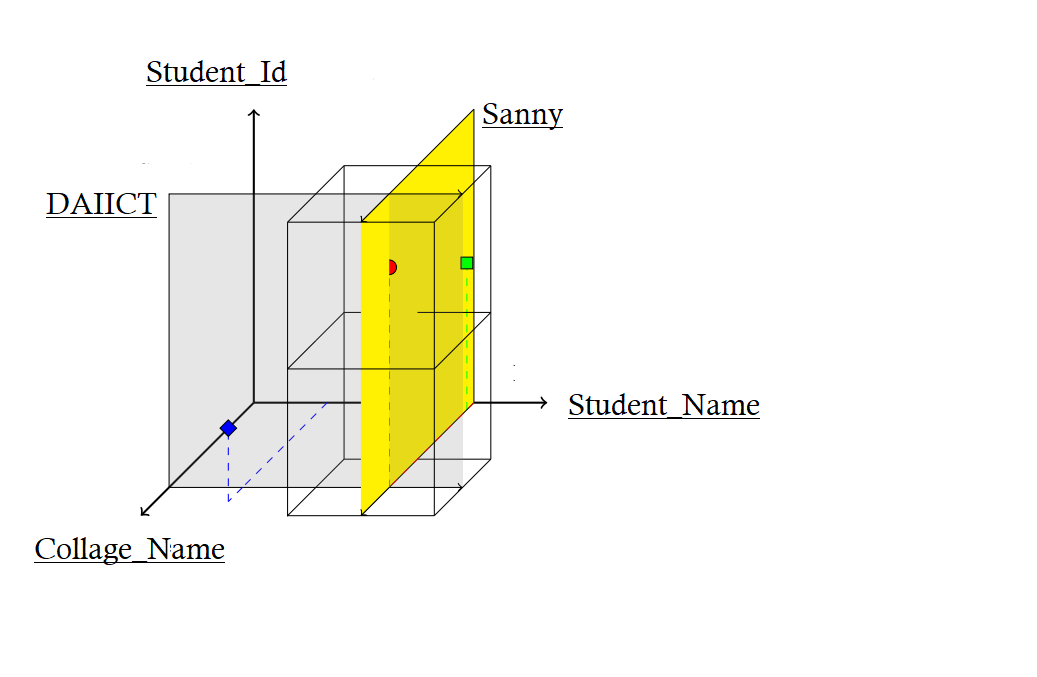
\includegraphics[width=0.95\linewidth]{
p1.png}\par 
\end{left}

\subsection{ Search Queries}

HyperDex uses geometric approach to find search Queries.HyperDex search a specific type of object using its attributes and value match with geometric axis and return the matched object. First of all hyperdex create a duplicate of  hyperspcae mapping and then through it execute search quarry. Now hyperdex map searches on hyperspace using mapping then determine intersection b/w given server region and resulting hyperplane then it search to only those server. we may get the result from this hyperplane.

\subsection{DATA PARTITIONING}
HyperDex’s Euclidean space construction are use to find how many needed server must be construct to find the matching object.hyperspace volume is exponentially increasing with the number of dimensions. for example if required searching secondary attributes are N so number of required server is O($ 2^N $).Hyperdex use data-partition for reduces the dimensional of the hyperspace and make it more efficiency search.HyperDex efficiently maintains consistency across subspace while maintaining a predictably low overhead.

\subsection{CONSISTENCY AND REPLICATION}
maintain consistency in Hyperspace is much complex  because hyperspace hashing map each object to multiple servers. Fro providing strong consistency and fault tolerance hyperdex use a novel technique called value dependent chaining in presence of concurrent updates .Hashing determining the current position of object replica on  different server nodes.change in signal object for consistency purpose change on all other replicas of object.
Such a scheme would at best provide eventual consistency because servers may receive updates out-of-order, with no sensible means of resolving concurrent updates.\\

hyperdex uses a replication to handle fault tolerance as traditional databases.It store duplicate copy of each within each region. let assume that we have three subspace called 0,1,2 and each have to replica of each data called h1 & h4 , h2 &h5, and h3 &h6. know we are updating data concurrently in all subspace and imaging if in second sub-space's first data replicas fails after some updates then the flow of data update continue but changes in that data  flow is that now it go through the second replica of it which is working fine. Also if first sub-space point leader fails then second replica of it data takes that stand. That is how the hyperdex provides us fault tolerance again certain failure scenario.\\

hyperdex provide us consistency guarantees. every action like get and put on any specific key are  linearizable whit all other key operation. so it is guarantees consistency. Also all search operation in hyperdex gives all data obj. which updated or insert at that time. lets take example of put it guarantees to give right output. if there is concurrent update at that time put gives committed object and also old object at same time.


\subsection{ HyperDex Server}
To achieve high performance HyperDex uses namely, edge-triggered,event-driven I/O techniques. The HyperDex server is structured around a concurrent, edge-triggered event loop wherein multiple worker threads receive network messages and directly process client requests.For avoiding or reducing probabilty of contention whenever possible here hyperdex uses lock-shading and lock free data-structure. but we uses array of locks here to protect per-key data-structures.Finally, the overheads associated with common operation such as hash-table and linked-list management  is reduced by uses of cache-conscious , constant-time data structures. 

\section{\textcolor{BurntOrange}{CONCLUSIONS}}
As we discuss above, we try to solve secondary indexing on any attributes and  also make it fast by use of hyperdex.This temp paper described high performance and scalability. Also consistency   and high availability in presence of partition failure scenario. We use hayper space hssing for it. We dicuss about it in details in this paper. Through this hyperdex provides additional functionality with all old database properties and performance.
\section{\textcolor{BurntOrange}{FUTURE SCOPE }}
 In future, we would like to do some research on how to implement this type of database and how to improve this functionality. We also want to use this type of database to see how it is different from other in real world. Here in this term paper we just discuss theoretical part of it and concept behind this database but in future we would going to do some performance test on how it better on secondary index quarrying  and how fast it is and also watch its through put on read and write operation. In general we would like to do some reserch on how it will implement and performance of every properties  of HyperDex. 
 
 



\begin{thebibliography}{}
\bibitem{a3} \url{https://www.cs.cornell.edu/people/egs/papers/hyperdex-sigcomm.pdf}
\bibitem{a4} \url{https://dbdb.io/db/hyperdex}
\bibitem{a5} \url{https://www.gsd.inesc-id.pt/~jgpaiva/pubs/sac14-presentation.pdf}
\end{thebibliography}
\end{document} %End of document
